% Figure: the admissible cone and its slices. Referenced from §7 after rem:extreme-rays;
% reused by §13's containment discussion. Pure TikZ. Design after the hub's
% memory_family_map.py (an inclusion diagram), adapted to this paper's cone.
%
% Pedagogic point: one picture of what Theorem 7.3 delivers. The outer region is the
% admissible cone (F of the form (7.1): drift b₀ ≥ 0 and a nonincreasing density k); its
% extreme rays (Prop. 7.7) are the Dickman rays Ein(τ·) and the pure delay s ↦ s, drawn on
% the boundary. Inside sits the Thorin subclass (k completely monotone), and the three
% distinguished families are slices cut through it by three different principles; the
% stable ray and the Bessel line meet at the heat-signaling member α = ½ — the one point
% the semigroup axioms allowed.

\begin{figure}[t]
\centering
\begin{tikzpicture}[every node/.style={font=\small}, line cap=round, >=stealth]

% the cone, drawn as a wedge from the apex F = 0
\coordinate (O) at (0,0);
\draw[thick] (O) -- (6.4,5.2);     % upper edge: the pure delay ray s ↦ s
\draw[thick] (O) -- (8.4,-1.2);    % lower edge: a Dickman ray Ein(τ ·)
\draw[thick] (6.4,5.2) .. controls (8.4,3.2) and (9.2,0.8) .. (8.4,-1.2); % the far boundary, Dickman rays
\node[anchor=west] at (6.55,5.1) {pure delay $F(s) = s$};
\node[anchor=west] at (8.55,-1.0) {Dickman rays $\mathrm{Ein}(\tau s)$};
\node[anchor=east] at (-0.15,0) {$F = 0$};
\node[anchor=west] at (-0.4,5.55) {\textbf{admissible cone}: $b_0 \ge 0$, $k$ nonincreasing};

% the Thorin subclass: k completely monotone
\draw[fill=gray!12,draw=gray!60] (O) -- (6.0,3.3) .. controls (7.2,1.9) and (7.3,0.4) .. (6.6,-0.3) -- cycle;
\node[gray!40!black,anchor=west] at (-0.4,-1.55) {shaded: the Thorin subclass, $k$ completely monotone};

% the three slices
\draw[very thick] (O) -- (8.2,2.9);
\node[anchor=west] at (8.85,2.9) {stable $s^{\alpha}$ (dilation symmetry)};
\draw[very thick,dashed] (O) -- (8.5,1.3);
\node[anchor=west] at (8.95,1.3) {Gamma $\gamma\log(1+s)$ (Thorin atoms)};
\draw[very thick,dotted] (1.6,3.1) .. controls (3.0,2.3) and (4.2,1.9) .. (6.2,1.6);
\node[anchor=south] at (1.6,3.15) {Bessel (locality)};
\fill (4.3,1.52) circle (2pt);
\node[anchor=north west] at (4.35,1.45) {$\alpha = \tfrac12$};

\end{tikzpicture}
\caption{The admissible cone. Theorem~\ref{thm:main-characterization} identifies the
exponents $F$ with pairs $(b_0, k)$, a drift and a nonincreasing density; these form a convex
cone (Lemma~\ref{lem:admissible-cone}) whose extreme rays are the Dickman rays
$\mathrm{Ein}(\tau\,\cdot)$ and the pure delay (Proposition~\ref{prop:extreme-rays}). Inside
it, the exponents with completely monotone $k$ form the Thorin subclass. None of the three
distinguished families of the paper is extreme; each is a slice cut by a different principle
--- the stable exponents $s^\alpha$ by dilation symmetry (Corollary~\ref{cor:semigroup-case}),
the Gamma family as the atoms of the Thorin representation, the Bessel family by locality
(\S\ref{sec:locality}) --- and the stable and Bessel slices meet at $\alpha = \tfrac12$, the
heat-signaling member, which is the one point the semigroup axioms allowed on the memory
line. The drawing is schematic: the cone is infinite-dimensional.}
\label{fig:admissible-cone}
\end{figure}
